%%
%% XPPAUT.tex
%% Login : <hoang-trong@hoang-trong-laptop>
%% Started on  Fri Oct  9 22:00:21 2009 Hoang-Trong Minh Tuan
%% $Id$
%% 
%% Copyright (C) 2009 Hoang-Trong Minh Tuan
%%

\chapter{XPP/XPPAUT tool}
\label{sec:xpp-tool}
\label{chap:XPPAUT}

In the previous chapter, you've learned a technique to visualize the
behavior of a dynamical system. This task, nowadays, can be done by
computer. One of those tool is XPP or the new version and new name XPPAUT.

\textcolor{red}{XPPAUT is a combined of XPP (for Phase Plane) and AUTO
  (a bifurcation program)} and was developed by Bard Ermentrout .
  
  
XPPAUT can do a lot of things (differential equations, delay
equations, volterra integral equations, discrete dynamical systems,
markov processes, bifurcation). XPPAUT is great for solving and
analyzing (numerically) ODEs (initial value problems, boundary value
problem, difference equations, delay equations...) Its application in
phase plane analysis is covered first and the bifurcation analysis.

{\bf Knowledge base}: For a {\it discrete dynamic system}, the state
at time point $n+1$ is dependent upon the previous state, i.e. the
common form is $X_{n+1} = F(X_n,n)$. In mostly examples and
applications, however, the {\it continuous dynamic systems} are more
common and is thus the concentration of this textbook. Due to its
continuity property, such systems need to use differential equation to
describe.
\begin{equation}
  \label{eq:121}
  \frac{dX}{dY}= F(X,Y)
\end{equation}
with $Y$ is the independent variable and is normally the time $t$,
i.e.
\begin{equation}
  \label{eq:349}
  \frac{dX}{dt}= F(X,t)
\end{equation}

In the previous chapter, you learned that in order to solve a
single differential equation, it needs
\begin{itemize}
\item the form of the equation, e.g. $F(X,t)$ which tells the rate of changes
of the system, e.g. the ODEs in normal form.


\item which symbols are dependent variables, e.g. X; which symbols are
  independent variables, e.g. t or Y here.

\item values of parameters

\item initial conditions, e.g. $X(0), X'(0)...$ (if it is initial
  value problem), boundary condition, e.g. $X(0), X(n)$ (if it is
  boundary value problem).

\end{itemize}

\textcolor{red}{In XPPAUT, users can specify all these stuffs in a single
  ASCII script file}.
The detail of the file is discussed in the next section.  XPP parser
will read this file to create machine usable code. Then, the methods
for solving, the graphics and all post-processing are all done using
the mouse and various menus, dialog boxes.

\section{Tool's information}
\label{sec:tools-information}

\subsection{Setting up}
\label{sec:setting-up}

You add these information into the \verb!~\.bashrc!
\begin{verbatim}
export XPPHELP=/usr/share/doc/xppaut/html/xpphelp.html
export BROWSER=/usr/bin/epiphany
\end{verbatim}


\subsection{Script file format}
\label{sec:file-format}

You model are described in a script file. Let's look at this sample
script to have a view of it.
\lstinputlisting{./codes/XPPAUT/ML_model.ode}


Here are some important notes when writing a script file.

\begin{enumerate}
\item A comment should be in a separate line and starts with
\verb!#!

\item Each statement starts with a command (e.g. {\it init}, {\it param},
...). The order of those commands are not important.

\item Each symbol (denoting dependent variables) can be singular
(X,Y...) or more characters (Ca, Buff...), don't use underscore (\_).

\item All symbols are case insensitive, e.g. ``vL'' is the same
as ``VL''

\item Dependent variables, not matter their symbols are, are
stored in an array name {\bf para}, whose index starts at zero,
i.e. para(0), para(1)...

\item A differential equation starts with {\it dX/dt=} command,
with ``$X$'' is the name of the dependent variable which is formed by
a set of characters, e.g. dCa, dBuff ...; $t$ here does not mean the
time, it denotes and independent parameter of $X$ and we cannot change
$t$ to a different symbol.

\item To set initial condition, use {\it init} command
  (e.g. {\it init V=0}) or use the statement of the form $para(0)=value$,
  e.g. $V(0)=1$.

\item To set values for parameters, use {\it par} or {\it param}
command

\item There must be no space in an assignment, e.g. x=2
(CORRECT), x = 2 (INCORRECT).


\item To end the script file, use the {\it done} command

\end{enumerate}

{\bf Example 1}: To describe this differential equation (the
electrostatistic of a passive membrane)
\begin{equation}
  \label{eq:122}
  C\frac{dV}{dt} = -g_L(V-V_L) + I_{app}
\end{equation}

\lstinputlisting{./codes/XPPAUT/pass_mem_model.ode}

{\bf Example 2}: To describe the predator-prey model
\begin{equation}
  \label{eq:259}
  \begin{split}
    \dot{x} &= x(x-x^2-y) \\
    \dot{y} &= y(x-1/u)
  \end{split}
\end{equation}
\lstinputlisting{./codes/XPPAUT/pred_prey_model.ode}

\subsection{Run tool}
\label{sec:run-tool}

After writing the script file for a model, you can now run XPPAUT with
the script as the command-line argument.
\begin{verbatim}
>xppaut filename.ode
\end{verbatim}
or it will ask you the ASCII file when you run the executable file
without any argument.


\subsection{GUI}
\label{sec:gui}

XPPAUT is a graphical user interface (GUI) for you to solve the
numerical problems described above. When you run it, a window will
show up as described in Fig.~\ref{fig:XPP_GUI}.

\subsection{Windows}
\label{sec:windows}


\begin{figure}[htb]
  \centerline{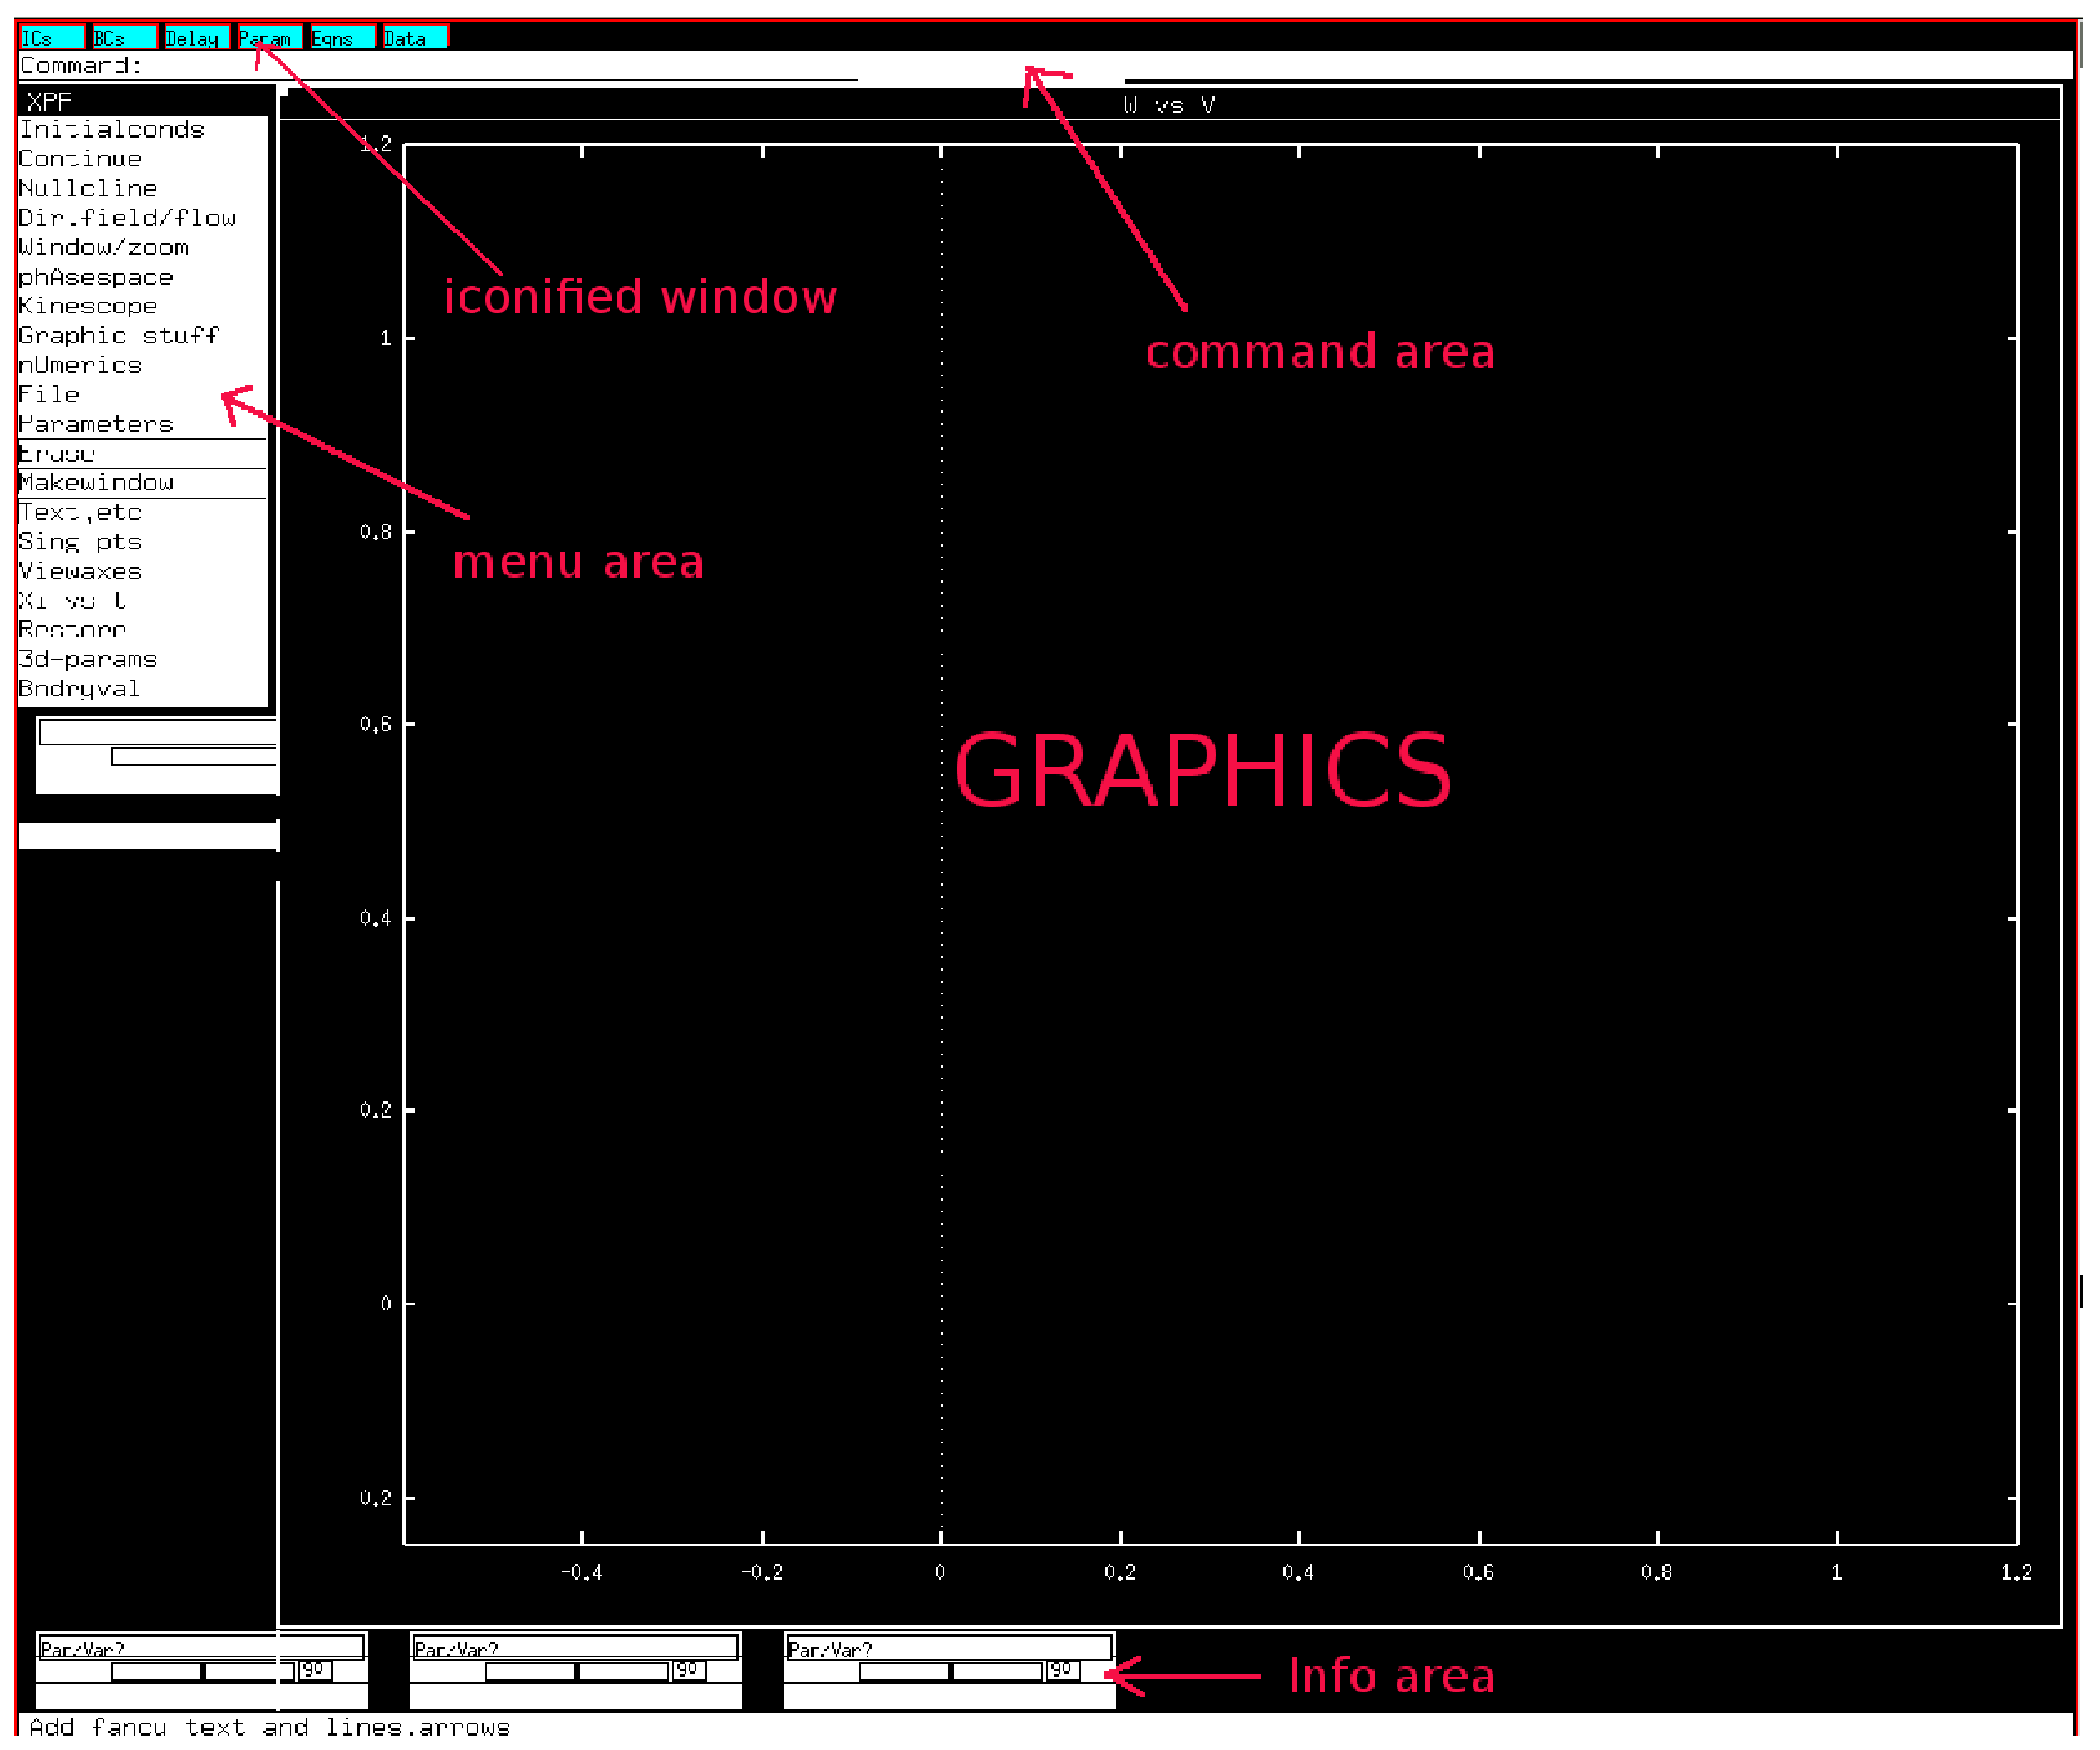
\includegraphics[height=10cm]{./images/XPP_GUI.eps}}
  \caption{The main window and its components}\label{fig:XPP_GUI}
\end{figure}

XPPAUT has 8 windows, 7 of which appear in the iconified fashion on
the top of the main window, as shown in Fig.~\ref{fig:XPP_GUI}. The
menu area display in a column-based on the left-side, which is
different from the conventional layout in many software.

Here are the list of the 7 iconified windows,
\begin{enumerate}
\item {\bf initial condition (ICs) window}

\item {\bf boundary conditions (BCs) window}

\item {\bf delay (Delay) window}

\item {\bf parameter (Param) window}: the 4-th icon on the top of the
  main window

\item {\bf equation (Eqns) window}

\item {\bf data browser (Data) window}

\item {\bf the command window}: where you can interactively type in
  and execute your command.
\end{enumerate}
Whenever you click on these iconified windows (except the command
window), some child-windows may pop up.

\subsection{Child-window (Dialog)}
\label{sec:dialog}

When you click on an iconified window, e.g. param window, a
child-window will pop up. There can be different types of control
element inside this child-window.

\begin{itemize}
\item To move from one textbox to another, press RET.
\item To select a control button, you still need a mouse.
\end{itemize}

\subsection{Using key combinations}
\label{sec:using-key-comb}


Besides using mouse to select a desired command,
\textcolor{red}{XPPAUT provides a convenient way to call all of these
  commands using key combinations}.

{\bf Example}: To Quit, click on File icon in the menu area, and select
Quit, press Y.  Hence, the key-binding to quit is FQY. It's easy to
remember. We will learn more from experiment.

\subsection{Solve the ODEs}
\label{sec:solve-odes-xppaut}

XPPAUT can perform solving numerical solution, e.g. for initial value
problems using various integration methods.  The very first thing you
have to decide is which numerical method that you want to use. You can
select the numerical method you want to perform the integration (read
Case study 8). If you press \underline{n(U)meric}-\underline{(M)ethod}
(key: UM), you will see a list of numerical methods: (D)iscrete,
(E)uler, (M)odified Euler, (R)unge-Kutta, (A)dams method, (G)ear
method, (V)olterra method, (B)ackEul (backward euler), (Q)ualst.RK4,
(S)tiff methods, (C)Vode method, DoPri (5) method, DoPri (8)3 method,
Rosen(2) 3 method, and s(Y)mplectic method.



{\it Integration} (key: IG) use the initial data and current numeric
parameters to find ``X'' if $dX/dt$ is known. Right after the
integration is done, the output is drawn in the graphics window, and
the data are saved for later use.

\begin{itemize}
\item {\it Adjust integrating range} The integration, of course, is
  carried out for a range of $t$, 0-20(ms) is default. You can extend
  the integration for a longer period of time, by clicking
  \underline{Continue} (key: C) or read the
  section~\ref{sec:change-xppa-defa}.


\item {\it Multiple integration}: With different initial conditions or
  parameters' values, you can carry out different integrations. This
  can be done by clicking \underline{InitialConds}-\underline{Range}
  (key: IR) which ask you for
\begin{verbatim}
Range over: V  # which parameter or variable to range over
Steps: 10      # how many steps (integrations) you take
Start: -100    # first and
End: 0         #    last point of the range
Reset storage (Y/N):   # won't store the last integration
Use old IC's (Y/N):
Cycle color (Y/N):
Movie (Y/N):
\end{verbatim}
  Here, you do integration with initial data (for V) from -100 to 0 mV
  in 10 steps (each step of 10mV).
  \begin{enumerate}
  \item Use reset storage (No) each integration is appended to
    storage, (Yes) only store the last integration. If the memory is
    exceeded, the integration will overwrite and stop.
  \item Use old IC's with (Yes) means to use the same initial
    conditions for each integration except for the variable that
    you're ranging (in the Range over), (No) use the final result of
    the previous integration as the initial condition for the next
    integration.
  \item Cycle color ask whether you want each trajectory (curve) to be
    in different colors.
  \item Movie asks you if you want to make a move from this loops or
    not (e.g. i=0..10).
  \end{enumerate}
\end{itemize}


{\bf Example}: Now, you can try to solve any of the models introduced
in the section \ref{sec:file-format}. First run the tool with the
given script file, then to solve the ODEs, click on
\underline{InitialConds} and then \underline{Go} (key: IG).
{\bf Result}: the ODEs is solved and the graph is plotted.  NOTE: To
clear the graph, press \underline{Erase} (key: E).

\subsection{Plot}
\label{sec:plot}

XPPAUT is so powerful that it allows you to plot the computed data.
When you solve the ODEs as described in section \ref{sec:solve-odes-xppaut},
by default, one dependent variable is plotted against $t$. To change
this to any pair of quantities you want, press
\underline{Graphics stuff}-\underline{Add curve} (key: GA); then
choose a new quantity for the y-axis. You will learn more in the next
section.

To obtain different curves, two things you would like to change are
values of {\it initial values} and {\it parameters' values}.

\begin{itemize}

\item {\it Load data for plotting} [optional]: When you open the Data
  Viewer window, if you have pressed IG, there will be existing
  data. However, you can load your own data by press Load button in
  the Data Viewer window.


\item {\it Plot}: By default, the x-axis is the independent value,
  which is normally $t$. When you press IG, a plot is automatically
  generated between the main dependent variable and $t$. However, you
  can choose to plot another quantity vs. $t$ by clicking on
  \underline{Xi versus t} (key:X).

  The independent variable, say $t$, can be switched to another
  parameter by clicking \underline{Viewaxes}-\underline{2D} (key: V2).

\item {\it  Axes ranges}: click
  \underline{Viewaxes}-\underline{2D} (key: V2) and then change the
  minimum/maximum value for x-axis, as well as the minimum/maximum
  values for the Y-axis. NOTE: The x-axis always start from zero.

  You can also click \underline{Window zoom}-\underline{Window} (key: WW).

\item {\it Redraw/Update}: Whenever you make change to the data, the
  graph/plot is not updated. To redraw/re-window the current graph so
  that it fits to the current window, click
  \underline{Window/zoom}-\underline{Fit} (key: WF).

\item {\it Zoom In/Out}:  click
  \underline{Window/zoom}-\underline{Zoom in} (key: WZ) or
  \underline{Window/zoom}-\underline{Zoom out} (key: WO).


\item {\it Axis label}: By default, there is no axis label, you can set
  them to clarify your graph by clicking
  \underline{Viewaxes}-\underline{2D} (key:V2). Click OK or type TAB
  to accept the new change.

\end{itemize}


(NOTE: On some displays, no rubber boxes are drawn for the zooming
operations. If this occurs, run with the {\bf -xorflag} option on the
command line.

\subsection{Multiple-curves in a single plot}
\label{sec:multiple-plot}


You can have multiple curves on the same figure (or window). It is
important that these different curve are of the same magnitude,
otherwise, the graph doesn't look good.

If you use the same data (i.e. single computation of the ODEs), this
can be done by choosing \underline{Graphics
  stuff}-\underline{Add
  curve}
(key: GA). However, if the different plots use different data
(e.g. multiple computation of ODEs based on different initial
conditions, or parameters' values), this can be done as a graphics
trick. We will discuss the later one.

This can be applied for you to draw a phase portrait, e.g. with
different initial conditions, or values of parameters, you may want to
plot those curves on the same figure.  Since XPPAUT always delete
data (i.e. the curve on window) after you update the data and perform
related calculations (e.g.  integration), you need to ``frezze'' the
old curve before making any change to existing data. By this way, the
old curves won't be deleted and then, you will have the chance to
overlay the new curve on the existing plot.

\begin{enumerate}
\item So, at first, make sure that the ranges of the two axes are of
  correct magnitudes for multiple curves.

\item To freeze it, click
  \underline{Graphics stuff}-\underline{Freeze}-\underline{Freeze}
  (key: GFF). A pop-up window asks you for the color (linetype), key
  name and curve name of the current curve. You have to select a color
  for it (from 0-10) as well as give it a name to discriminate it with
  other new curves.

\begin{itemize}
\item The color can be either  0 (white) or 1-9 (red-blue). It means
  you can have maximum 10 curves on a single plot. This is more than
  enough. 

\item The curve name is for easy reference and should be a few
  characters (or you can let it default).

\item The key name is the {\it legend} of the curve - what will be
  printed on the graph. A key on a graph consists of a line followed
  by some text describing the line (maximum 15 characters). The key
  can be turned on or off by clicking
  \underline{Graphics stuff}-\underline{Freeze}-\underline{Key} (key:
  GFK). You can also use the mouse to relocate the position of the
  ``on'' key.
\end{itemize}

\item After the first curve is freezed, you can freely update the
  \hyperref[sec:parameters]{parameter} or
  \hyperref[sec:initial-values]{initial conditions} before you
  recompute (e.g. integrate) the unknown parameter and draw it
  (X). You can also freeze this curve (follow the same procedure) if a
  third curve is needed.

\item Finally, to display the legend of each curve, you turn on all
  keys by pressing GFKK, and use the mouse to point to the place where
  you want to put the key (legend).

\end{enumerate}

To remove the last added curve to the plot, you click
\underline{Graphics stuff}-\underline{Delete last} (key: GD).


\subsection{Multiple plots}
\label{sec:many-plots}

You can also have more than one figure at the same time. To create a
new figure (the current plot is copied to the new figure also), you
click \underline{Makewindow}-\underline{Create} (key: MC). If the
trajectories are not displayed, you click \underline{Restore} (key: R)
to show them again.

When more than one figure, the active one has a white square on the
upper left corner. You can active any figure by clicking on it. To add
a curve to the active figure, you click \underline{Xi vs t} (key: X)
and choose the new quantities, new plot will be displayed
automatically. To get a different scale, you can experiment with
\underline{Window/zoom} or \underline{Viewaxes}-\underline{2D}.

You can also delete (destroy) the active figure by using
\underline{Makewindow} (key: H) and

(K) kill all but the main window

(D) destroy the current active window (except the main window)

(B) put the active window on the bottom


\subsection{Initial values}
\label{sec:initial-values}

To change the initial data, use (1) the {\it ICs window} and then
click \underline{Initialconds}-\underline{Go} (key:IG) to integrate);
(2) click \underline{Initialconds}-\underline{New} (key: IN) for new
initial data and the integration is automatically computed.

(I) provides other choices: (N)new initial data and then integrate,
(G)use the current initial conditions to integrate, (L)use the end
values of the last integration as the start of a new one.

\subsection{Parameters}
\label{sec:parameters}

Parameters are symbols to represent a constant. These information are
not accessible to the user so they cannot be plotted, but they can be
used in formulas. 

To change the values for the parameters, use (1) the
{\it Param window}, (2) in the main window, press P and then type the
name of the parameter to adjust; finally, you type the new value for
the parameter.


This is rarely used, however, you can also make a fixed scalar
(specified by one parameters) for plotting by adding an auxiliary that
is equal to that parameter.

\begin{lstlisting}
aux myr=R
\end{lstlisting}


\subsection{Data manipulation}
\label{sec:data-manipulation}


Whenever you open a model with XPPAUT, the data are not generated. 
\begin{itemize}

\item {\it Generate the data}: You can press (I)ntegrate and choose
  (G)o, i.e (I)(G). and the set of ODEs will be solved. The default
  range for the independent variable is from [0..20]. However, you can
  change it, see {\it range for independent variable}.

\item {\it See the data}: use Data Browser/Viewer window (the 6-th
  icon on the top of the main window)


\item {\it Create formulated data} (auxiliary data, temporary data):
  By default, in the Browser/Viewer just display the computed data for
  $t$, and any other dependent variables. However, You can add a new
  column whose values are computed from a given formula, using the
  {\bf AddCol} button in the Data Viewer window. You can define this
  in the script, see \hyperref[sec:auxil-temp-quant]{this section}.

\item {\it Range for independent variable}: By default, dX/dt is
  solved for the $t$ in the range [0,20]. However, you can extend $t$
  to any value by changing its continue value: (1) Click on the
  ``continue'' menu item in the menu area; (2) press C, and then type
  the new value.


\item {\it Restrict the data to be plotted}: You don't have to use all
  the data in the plot, you can manually select the initial value and
  the last value by using First and Last feature in the Data Viewer
  window. Then, you can replot the data marked by First and Last, by
  pressing Restore in the Data Viewer window.

\end{itemize}




\subsection{Export the data}
\label{sec:export-data}


\begin{itemize}
\item {\it Save the data} [optional]: You can save the existing data
  in the Data Viewer window for later use or plotting with any other
  tools. 

\item {\it Export numeric data} You can save data in tabulated
format that can be used by XPP as a function or inputs. You open the
Data Viewer window, use First and Last to mark the desired data you
want to save, you then be prompted for Column name, the min and max
you want your independent variables to range and the file name.

\item {\it Save numeric data} This time, you can save all to a
file by choosing Write in Data Viewer window.
\end{itemize}

\subsection{Export figure}
\label{sec:export-figure}


{\it Save}: To save the figure to a PostScript file, click
\underline{Graphics stuff}-\underline{Postscript} (key: GP) - a pop-up
window ask you some parameters

\begin{verbatim}
BW-0/Color-1
Land (0) / Port(1)
Axes font size
Font: Times-Roman
Linewidth: 5
\end{verbatim}
and finally you type the file name in the command area.



\subsection{Change XPPAUT default options}
\label{sec:change-xppa-defa}

You can change the XPPAUT default options by declaring some directive
in the script file. These lines should start with the at sign
(@). This will help you to adjust the setting that fit to your script
without needing to do it every time you run it.

{\bf Example}: Set the x-axis to be the $V$ variable,  the y-axis to
be the $w$ variable, the range of values in each axis, the total
amount of integration to be 100. Finally, since XPPAUT allocates
memory only enough to store 4000 time points only, you can make it
allocated as much as you want, with $maxstor$ setting.

\begin{lstlisting}
@ xp=V, yp=w, xlo=0.25, xhi=1.25, ylo=-.5, yhi=1, total=100
@ maxstor=10000
\end{lstlisting}

{\bf Example}: 
\begin{lstlisting}
@ meth=euler, dt=.1, total=1000, bound=1000, nout=400
@ trans=1000
\end{lstlisting}

You can set them permanently by using the resource file \verb!.xpprc!
in your \verb!$HOME$! directory, for example
\begin{verbatim}
@ but=quit:f q
@ maxstor=5OOOO,bell=0
@ meth=qualrk,tol=le-6,atol=le-6
\end{verbatim}
which does
\begin{itemize}
\item put a QUIT button on the top bar
\item allocate 50,000 storage points (otherwise the default is 5000), turn BELL off
\item make the default integrator is adaptive Runge-Kutta
\end{itemize}

\subsection{Supported functions}
\label{sec:supported-functions}

With XPPAUT, you can use the following functions in your formula, as
shown in Table~\ref{tab:xppaut_func}.
\begin{table}[tbh]
  \centering
  \begin{tabular}{|c|c|}
    sin(x) & cos(x) \\
    tan(x) & atan2(x,y), i.e. $tan^{-1}(y/x)$ \\
    asin(x), i.e. $sin^{-1}(x)$ & acos(x) \\
    sinh(x) & cosh(x) \\
    max(x,y) & tanh(x) \\
    atan(x), i.e. $tan^{-1}(x)$ & x**y, or x\^{}y \\
    exp(x) & abs(x) \\
    log10(x),  i.e. $log_{10}(x)$ & sqrt(x), i.e. $\sqrt{x}$\\
    min(x,y) & sign(x), i.e. $x/|x|$ \\
    flr(x), i.e. $int(x)$ & erfc(x), i.e. $1-erf(x)$ \\
    erf(x), i.e. $erf(x)$ & mod(x,y), i.e. x modulo y\\
    ln(x) or log(x), i.e. $ln(x)$ & heav(x), i.e. 1 if $x\ge 0$; else
    0 \\
    x | y, i.e. x OR y & not(x) \\
    bessely(n,x), i.e. $Y_n(x)$ & besselj(n,x), i.e. $J_n(x)$
  \end{tabular}
  \caption{Names of standard XPPAUT function}
  \label{tab:xppaut_func}
\end{table}

Other functions include:
\begin{enumerate}
\item $ran(x)$ generate a uniformly distributed random number

\item $normal(x,s)$ generate a normally distributed random number with
  mean $x$ and standard deviation $s$.

\item if(x)then(y)else(z): return $y$ if $x$ is true; otherwise return
  $z$

\item sum(x,y)of(z) : with $z$ is some expression involving the index
  $i$, then it return $\sum_{i=x}^{i=y}z$.
\end{enumerate}

Here are more complicated functions:


\subsection{User-defined function}
\label{sec:user-defin-funct}

You can define a function in XPPAUT in an intuitive way
\begin{lstlisting}
func_name(parameters)=formula
\end{lstlisting}
Example:
\begin{lstlisting}
f(x,y)=x^2+x-4
\end{lstlisting}

A function can depend on another function
\begin{lstlisting}
f(x,y)=x*g(y,3)
g(x,y)=x^2+4*y
\end{lstlisting}

Be careful when you define a recursive function, follow this guide
\begin{lstlisting}
fac(x)=if(x>0)then(x*f(x-1))else(1)
\end{lstlisting}


\subsection{Auxiliary and temporary quantities}
\label{sec:auxil-temp-quant}

You have learnt about the concept of auxiliary quantities in the
section \ref{sec:data-manipulation}. However, such quantities are not
automatically generated by default. After reading and running the
script, the data that you receive are from the dependent
variables. However, you can also have data that are generated from
these variables. This can be done in XPPAUT script with the {\bf aux}
command
.
\begin{lstlisting}
aux stuff=x+y*sin(t)
\end{lstlisting}
with $x, y, t$ are all variables.

The important point is that auxiliary quantities are not know to
XPPAUT, so you cannot use it in any formulas.


\subsection{Discontinuous differential equations}
\label{sec:disc-diff-equat}

{\it Discontinuous differential equations}: Suppose that you want to
``reset'' the value of the variable $V$ to zero once it hits some
value $V_t$.

XPPAUT use {\bf global flags} with the general syntax
\begin{lstlisting}
global sign condition {event1; event2;...}
\end{lstlisting}
the {\it condition} is evaluated each time step of the integrator. If
the {\it sign} is 1 and the {\it condition} changes from negative to
positive, or if the {\it sign} is -1 and the {\it condition} changes
from positive to negative, then each of the {\it events} is
performed. The {\it events} can be only in the form of assignments,
i.e. $x=expr$ with $x$ is one of the variables and $expr$ is some
expression.

{\bf Example}: The integrate-and-fire model for a neuron
\begin{equation}
  \label{eq:284}
  \frac{dV}{dt}=I-V
\end{equation}

The code is
\lstinputlisting{./codes/XPPAUT/int-fire_model.ode}

\subsection{Misc}
\label{sec:misc}


\textbullet {\it Bell}: to turn of the noisy bell sound, (F)(B)

\section{Case studies}
\label{sec:case-studies}

\subsection{Case study 1 - multiple-curve adjust parameters' values}
\label{sec:case-study-1}

Here, you continue with example 1.

\begin{enumerate}
\item Now, you run XPP, tell it the path to the ASCII source file then press
RET or can specify it directly on the command line

\begin{verbatim}
$xppault ode/passive_membrane.ode
\end{verbatim}

The equation you have is

\begin{equation}
  \label{eq:123}
  \frac{dV}{dt} = \left[ -g_L(V_m-V_L) + I_{app} \right]/C
\end{equation}
To study the time evolution of this system, i.e.  the time evolution
of the voltage, you need to integrate the above equation.

\item Compute the integration (trajectory), e.g. finding V(t), key
  IG. Here you dont' care which method XPP used to compute the
  integration until \hyperref[sec:case-study-8]{CS 8}. The two common
  methods are Euler method and Runga-Kutta method.

  The plot of the voltage V(t) vary over time is automatically
  plotted.  What do you see? - an exponentially decaying solution
  (voltage vs. time)

\item Freeze the existing curve (key: gl=2, color=5), and change the
  parameter, e.g. gL from 2 to 4, and reintegrate the equation. Then,
  freeze the new curve (key: gl=4, color=0). Finally, turn on the
  key. What do you see?  - a plot with 2 curves.

\item Save the plot to a postscript file
  (e.g. \verb!ps_images/p_mem_gL.ps!) with key GP.
\end{enumerate}


\subsection{Case study 2 - replot by adjusting the range}
\label{sec:case-study-2}

Here, you continue with example 1 and learn how to adjust initial data.

\begin{enumerate}
\item Run XPP with \verb!passive_membrane.ode!

\item Set $I_{app}=0$, $V(0) = 30$ and integrate.

\item Change the time range for 20 more milliseconds (until 40). To
  replot, press (X)

\item As the rest state is at -60mV, you will integrate with initial
  voltage as -100mV, -90mV, ..., 0mV (e.g. from -100mV to 0mV in 10
  steps). 

Set the axis range $V=-100 \rightarrow 0$mV, $t=0\rightarrow 20$ms.

Perform the series of integration by pressing (I)(R)
\begin{verbatim}
Range over: V  # which parameter/variable to vary
Steps: 10      # how many steps you take
Start: 0       # first and
End: -100      #    last point
Reset storage (Y/N):y
Use old IC's (Y/N):y
Cycle color (Y/N):y
Movie (Y/N):n
\end{verbatim}
\end{enumerate}

\subsection{Case study 3 - create auxiliary data}
\label{sec:case-study-3}

The previous case studies show you the actual trajectories (the
curve). Of course, this curve has been plotted using existing numeric
data. This data can also be save to the file for further usage.

This CS continue with the CS 2

\begin{enumerate}
\item Open Data Viewer window

\item Find the voltage at $t=12$. 

\item Find the approximate time at which $V=-30mV$.

\item Add a new column (called IL) to compute the total leak current
  $g_L(V_m-V_L)$.

\item Plot the total leak current as a function of time.

\item Save (write) the data to a file
\end{enumerate}

\subsection{Case study 4 - nullclines}
\label{sec:case-study-4}

Here, you will learn to determine the fixed point and its stability.
\begin{enumerate}
\item Change the current $I_{app}=20$

\item Determine the fixed point, you click \underline{Singl pts}
(singular point) - \underline{Go} (key: SG).

\item Repeat with $I_{app}=-15$.

\item You can try with different initial conditions or different
  values of $g_L$.
\end{enumerate}

\subsection{Case study 5* - review}
\label{sec:case-study-5}

Here, you review the previous techniques
\begin{equation}
  \label{eq:124}
  C\frac{dV}{dt} = -g_L(V_m-V_L) + I_{app} + A \sin(\omega t)
\end{equation}

\begin{enumerate}
\item Edit the new ASCII script file for the above equation
$A=50, V_L = -60$mV, $I_{app} = 0$.
\item Run XPP with this new file

\item Plot the instantaneous current ($I_L=\frac{V-V_L}g_L$) and the
  voltage on the same plot (use (V)(2)). What do you see? - voltage
  trail the current in a linear manner.
\end{enumerate}

\begin{verbatim}
# Passive membrane
v(0)=-60
par C=20 gL=2 vL=-60 i=0 w=3 A=50
dv/dt=(-gL*(v-vL) + i + A * sin(w*t))/c

done
\end{verbatim}
\subsection{Case study 6 - user-defined function + aux. data}
\label{sec:case-study-6}

A more realistic model of the membrane is given by adding a new term
for calcium conductance
\begin{equation}
  \label{eq:125}
  C\frac{dV}{dt} = I_{app} - g_L(V_m-V_L) - g_{\ce{Ca}}m_\infty(V_m) (V_m-V_{\ce{Ca}})
\end{equation}
with the ratio of open channels is a function of membrane voltage
\begin{equation}
  \label{eq:126}
  m_\infty(V_m) = .5 (1 + \tanh (\frac{V_m-V_1}{V_2}))
\end{equation}
You can read sec.~\ref{sec:exampl-ionic-curr}.

How can this be written in the form of XPP script file
\begin{verbatim}
# One fast persistent calcium channel
# Here is the equation
dv/dt=(i+gl*(vl-v)+gca*minf(v)*(vca-v))/c

#and the initial condition
V(0)=-60

# and the calcium current
aux ica=gca*minf(v)*(v-vca)

# and the parameters
param vl=-60,vca=120
param i=0,gl=2,gca=4,c=20
param v1=-1.2,v2=18

# and the functions
minf(v)=.5*(1+tanh((v-v1)/v2))
done
\end{verbatim}

The new things are
\begin{itemize}
\item {\it auxiliary quantities}: new data columns that we discussed in CS
  4 now can be specified in the script file using {\bf aux} command
  followed by the formula

\item {\it user-defined functions}: a function has the form
  $func\_name(para1,para2)=expression$
\begin{verbatim}
minf(v)=.5*(1+tanh((v-v1)/v2))
\end{verbatim}

\item {\it fixed quantities}: fixed quantities function as
  intermediate quantities to be used in other expressions. The
  statement has the form {\it name=formula}, and must be evaluated before
  the right-hand side of the expression that utilizes it.

The faster version of the script
\begin{verbatim}
# Here is the equation
dv/dt=(i+gl*(vl-v)-icaf)/c

#and the initial condition
V(0)=-60

# and the calcium current as a fixed quantity
icaf=gca*minf(v)*(v-vca)

# make ica available to look at
aux ica=icaf

# and the parameters
param vl=-60,vca=120
param i=0,gl=2,gca=4,c=20
param v1=-1.2,v2=18

# and the functions
minf(v)=.5*(1+tanh((v-v1)/v2))
done
\end{verbatim}
\end{itemize}

\subsection{Case study 7* - review}
\label{sec:case-study-7}


Tasks:
\begin{enumerate}
\item Add new auxiliary quantity ``leak current'' $g_L*(V_m-V_L)$
\end{enumerate}

\begin{enumerate}
\item Rewrite this nonlinear pendulum as a pair of first-order
  differential equations
  \begin{equation}
    \label{eq:127}
    ml\frac{d^2x}{dt^2} = -ml\sin(x) - f\frac{dx}{dt}
  \end{equation}
with
\begin{equation}
  \label{eq:128}
  E = \frac{1}{2}ml^2 (\frac{dx}{dt})^2 + mgl(1-\cos(x))
\end{equation}
\end{enumerate}

\begin{verbatim}
dx/dt=v  
dv/dt=sin(x)-f*v/(m*l)

x(0)=4 
param m=3 l=2 f=5

done
\end{verbatim}

This is another task
\begin{enumerate}
\item Write an ODE for the single variable continuous time Hopfield
  model
  \begin{equation}
    \label{eq:129}
    \tau\frac{da}{dt} = -a + \omega f(a) + i
  \end{equation}
with 
\begin{equation}
  \label{eq:130}
  f(a) = 1/(1+e^{-\beta(a-\theta)}
\end{equation}
given $\beta=2, \theta=1, i=0, \tau=1, \omega=1, a(0)=0$.
\end{enumerate}
\begin{verbatim}
param tau=1 theta=1 beta=1 w=1 i=1
a(0)=0

f(a)=1/(1 + exp(-beta*(a-theta)))
da/dt=(-a + w * f(a) + i)/tau

done
\end{verbatim}

\subsection{Case study 8 - numerical methods}
\label{sec:case-study-8}

Here, you will learn how you can calibrate the settings for  numerical
algorithms. You press n(U)merics. Here is the information for
sub-items. 

\begin{enumerate}
\item {\it Bound}: maximum possible value for the variable,
  e.g. V. Default is 100, however, as membrane potential can reach up
  to 120mV, then you should adjust it to 1000 by pressing (B).

\item {\it Total}: the time range, is 20ms by default. If you want to
  integrate for at least 200ms, press (T) total

\item {\it Dt}: this is the time-step for integration (default is
  0.05). The smaller $dt$, the more precision the
  computation. However, for our example, set it to .2 by pressing (D).

\item {\it n(O)ut}: not all values of V(t) are outputted on the plot,
  you can tell how frequently you want output to plot and browse. The
  default is 1 (use every computed value), e.g. if Dt=0.05 you will
  get the new value every 0.05ms.

\item {\it t(R)ansient}: 

\item {\it Start time}: the starting time, set to 0 by default. In
  {\it autonomous} differential equations, as there is no time factor, it is
  totally irrelevant and can get negative value. 

\item {\it Method}: default method is {\bf Adams-Bashforth} predictor
  corrector.

Gear method is only presently available in XPP (use an adaptive step
size - it can change)

Modified Euler is also called Heun's method.
\end{enumerate}

\begin{figure}[htb]
  \centerline{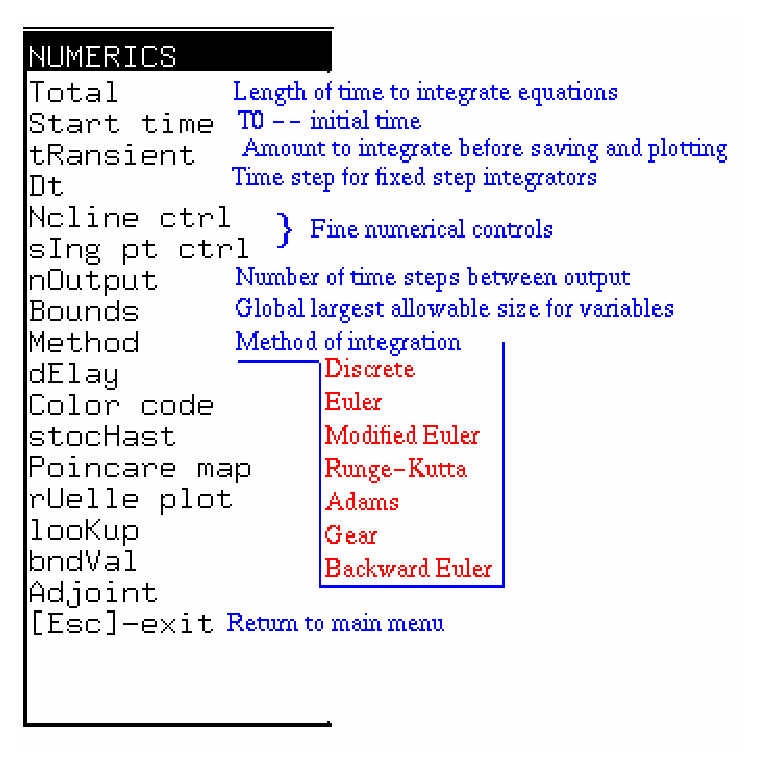
\includegraphics[height=7cm]{./images/XPP_numcom.eps}}
  \caption{Numerical settings for XPP}\label{fig:XPP_numcom}
\end{figure}

This case study use the equations in the previous case study.
\begin{verbatim}
2
# the number of things to plot is 2

# declare the variables setting v(0) to rest
variable v=-60

# declare other stuff to plot
aux ica

# declare the parameters
param vl=-60,vca=120
param i=0,gl=2,gca=4,c=20
param v1=-1.2,v2=18

# user defined functions 
user minf 1 .5*(1+tanh((arg1-v1)/v2))

# right-hand sides of ODES in order of declaration
odev (i+gl*(vl-v)+gca*minf(v)*(vca-v))/c

# definitions of auxiliary quantities in order of declaration
oica gca*minf(v)*(v-vca)

done
\end{verbatim}

Next, set the window size: x-axis $0..200$, y-axis $-150..150$.  After
adjusting the parameters, you can do the integration by pressing
(I)(G).


The result is a straight-line as the system essentially starting at
rest. Now, change the initial condition to $-20$mV. What do you see? -
a decay to the rest state.


Let's see with a different initial voltage $V_m=-10$mV. What do you
see? - the voltage increases to a new level of around 50mV. This is an
example of {\it multi-stability}. 

This suggest that between -20mV and -10mV there must be a critical
value  of voltage which acts as a threshold and any potential below
this goes to the low state and above goes to the high state. 

{\bf NOTE}: Non-linear systems are often characterized by the
existence of multiple stable behaviors.

\subsection{Case study 9 - multiple figures}
\label{sec:case-study-9}

In this CS, you learn how to create a copy of the existing window.
Press (H)(C) to create the copy figure. With this new window, draw ICA
vs. time, by pressing (X) and choose ICA.
What do you see? - negative value for $I_{\ce{Ca}}$, so it is an inward
current. The point at which the calcium current is most negative can
be examined approximately using the mouse to right-click at the lowest
point (about 4.6ms).

\subsection{AUTO}
\label{sec:auto}

The study of the parametric dependence of differential equations is
called {\bf continuation} and the analysis of how solution
appear/disappear as parameters vary is called {\bf bifurcation theory}
from the Latin word {\it bifurkus} = branching.

AUTO is one of the best {\it continuation} packages available. The
behavior of the system is a function of parameters. AUTO is now a part
of XPP.

To use AUTO, you have to write a script file, starting at a known
steady state.

\subsection{Case study 10}
\label{sec:case-study-10}

Here, a more realistic model of the membrane is discussed, the
``Morris-Lecar'' model. Besides the inward calcium current, there
should be the outward potassium current.

\begin{verbatim}
dv/dt = (-gl * (v - vl) - gca * minf(v) * (v-vca) - gk * w * (v - vk)
+ i)/C
dw/dt = lambw(v) (lambinf(v) - w)

winf(v)=0.5 * (1+tanh((v-v3)/v4))
lambinf(v)=phi * cosh((v-v3)/(2*v4))

\end{verbatim}


\subsection{Summary }
\label{sec:summary-}


XPP can handle up to 590 differential equations. There can be up to 10
graphics window to be visible at once. Figure can be exported as a
postscript file. 

Post-processing is easy: histograms, FFT and applying functions to
columns of the data.

Equilibria and linear stability can be computed.



If XPP is in the middle of a calculation, and you want to halt that
operation, press Esc key, in some case,
you need to type the slash (/) key on the keyboard.


%%% Local Variables: 
%%% mode: latex
%%% TeX-master: "mainfile"
%%% End: 
